
\documentclass[letterpaper,10pt,english]{hitec}

%\usepackage{cmap}
%\usepackage[T1]{fontenc}
\usepackage{amsmath,amssymb,amstext}
\usepackage{babel}
%\usepackage[utf8]{inputenc}
\usepackage{graphicx}
\usepackage{hyperref}



\title{lwHAL Documentation}
\date{June 5th, 2021}
%\release{0.00}
\author{S.Furlan}
%\makeindex

\begin{document}

%\pagestyle{empty}
\maketitle
\blinddocument
\newpage

%\pagestyle{plain}
\tableofcontents
%\pagestyle{normal}

\newpage

\section{light-weight Hardware Abstration Layer - lwHAL}

\newpage

\section{Target ports}
\subsection{STM32F4xx}
We tested the lwHAL on the STM NUCLEO-F429ZI development board. The test consists
in turning the red LED on and then toggling at every second the green LED on the board.

We initialized a new project for the NUCLEO-F429ZI from the STM IDE, setting
with default configuration. Then we added the lwHAL folder inside the $/Core$, as
shown in figure \ref{fig:stm_ide}.
The $\#define$ $STM32F4xx$ must be uncommented in the $src/config.h$.
Make sure to include the path to the lwHAL folder inside the IDE.

Copy the code snippets from the
$ports/stm32f4/stm32f4\_test.c$
into the $main.c$.
Compile and run the binary on the board. You will see the red LED turning on and
the green LED blinking at a frequency of 1 Hz.

\begin{figure*}[ht]
\centering
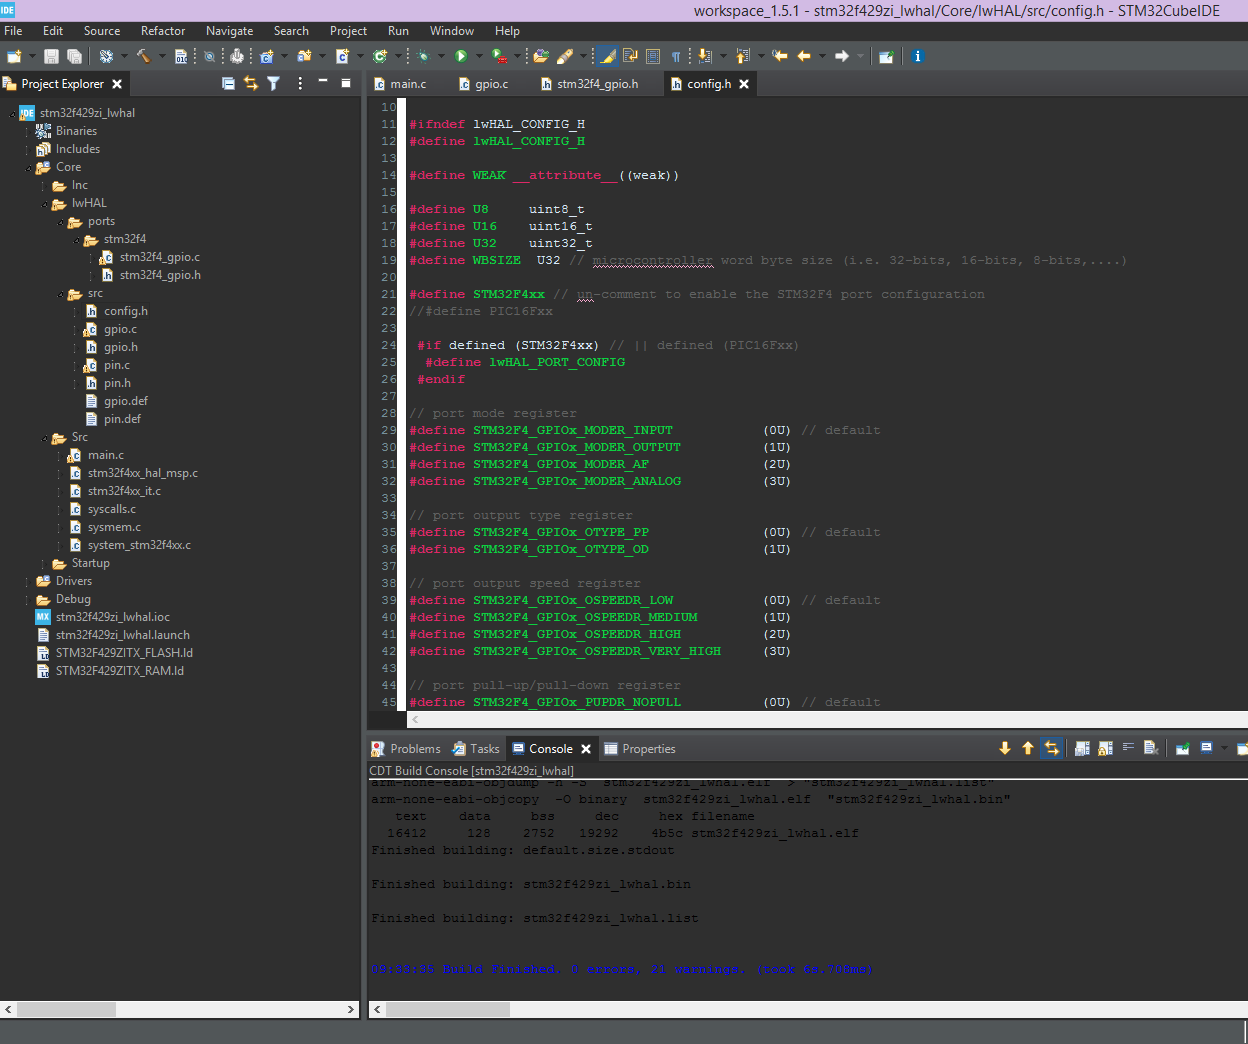
\includegraphics[scale=0.4]{stm_ide.png}
%\caption{}
\label{fig:stm_ide}
\end{figure*}

\newpage

\section{lwHAL license information}

The MIT License (MIT)
\\
\\
Copyright (c) 2021 Silvano Furlan, and others
\\
\\
Permission is hereby granted, free of charge, to any person obtaining a copy
of this software and associated documentation files (the “Software”), to deal
in the Software without restriction, including without limitation the rights
to use, copy, modify, merge, publish, distribute, sublicense, and/or sell
copies of the Software, and to permit persons to whom the Software is
furnished to do so, subject to the following conditions:
\\
The above copyright notice and this permission notice shall be included in
all copies or substantial portions of the Software.
\\
\\
THE SOFTWARE IS PROVIDED “AS IS”, WITHOUT WARRANTY OF ANY KIND, EXPRESS OR
IMPLIED, INCLUDING BUT NOT LIMITED TO THE WARRANTIES OF MERCHANTABILITY,
FITNESS FOR A PARTICULAR PURPOSE AND NONINFRINGEMENT. IN NO EVENT SHALL THE
AUTHORS OR COPYRIGHT HOLDERS BE LIABLE FOR ANY CLAIM, DAMAGES OR OTHER
LIABILITY, WHETHER IN AN ACTION OF CONTRACT, TORT OR OTHERWISE, ARISING FROM,
OUT OF OR IN CONNECTION WITH THE SOFTWARE OR THE USE OR OTHER DEALINGS IN
THE SOFTWARE.


\end{document}
